\documentclass[twoside]{book}

% Packages required by doxygen
\usepackage{fixltx2e}
\usepackage{calc}
\usepackage{doxygen}
\usepackage[export]{adjustbox} % also loads graphicx
\usepackage{graphicx}
\usepackage[utf8]{inputenc}
\usepackage{makeidx}
\usepackage{multicol}
\usepackage{multirow}
\PassOptionsToPackage{warn}{textcomp}
\usepackage{textcomp}
\usepackage[nointegrals]{wasysym}
\usepackage[table]{xcolor}

% Font selection
\usepackage[T1]{fontenc}
\usepackage[scaled=.90]{helvet}
\usepackage{courier}
\usepackage{amssymb}
\usepackage{sectsty}
\renewcommand{\familydefault}{\sfdefault}
\allsectionsfont{%
  \fontseries{bc}\selectfont%
  \color{darkgray}%
}
\renewcommand{\DoxyLabelFont}{%
  \fontseries{bc}\selectfont%
  \color{darkgray}%
}
\newcommand{\+}{\discretionary{\mbox{\scriptsize$\hookleftarrow$}}{}{}}

% Page & text layout
\usepackage{geometry}
\geometry{%
  a4paper,%
  top=2.5cm,%
  bottom=2.5cm,%
  left=2.5cm,%
  right=2.5cm%
}
\tolerance=750
\hfuzz=15pt
\hbadness=750
\setlength{\emergencystretch}{15pt}
\setlength{\parindent}{0cm}
\setlength{\parskip}{3ex plus 2ex minus 2ex}
\makeatletter
\renewcommand{\paragraph}{%
  \@startsection{paragraph}{4}{0ex}{-1.0ex}{1.0ex}{%
    \normalfont\normalsize\bfseries\SS@parafont%
  }%
}
\renewcommand{\subparagraph}{%
  \@startsection{subparagraph}{5}{0ex}{-1.0ex}{1.0ex}{%
    \normalfont\normalsize\bfseries\SS@subparafont%
  }%
}
\makeatother

% Headers & footers
\usepackage{fancyhdr}
\pagestyle{fancyplain}
\fancyhead[LE]{\fancyplain{}{\bfseries\thepage}}
\fancyhead[CE]{\fancyplain{}{}}
\fancyhead[RE]{\fancyplain{}{\bfseries\leftmark}}
\fancyhead[LO]{\fancyplain{}{\bfseries\rightmark}}
\fancyhead[CO]{\fancyplain{}{}}
\fancyhead[RO]{\fancyplain{}{\bfseries\thepage}}
\fancyfoot[LE]{\fancyplain{}{}}
\fancyfoot[CE]{\fancyplain{}{}}
\fancyfoot[RE]{\fancyplain{}{\bfseries\scriptsize Generated by Doxygen }}
\fancyfoot[LO]{\fancyplain{}{\bfseries\scriptsize Generated by Doxygen }}
\fancyfoot[CO]{\fancyplain{}{}}
\fancyfoot[RO]{\fancyplain{}{}}
\renewcommand{\footrulewidth}{0.4pt}
\renewcommand{\chaptermark}[1]{%
  \markboth{#1}{}%
}
\renewcommand{\sectionmark}[1]{%
  \markright{\thesection\ #1}%
}

% Indices & bibliography
\usepackage{natbib}
\usepackage[titles]{tocloft}
\setcounter{tocdepth}{3}
\setcounter{secnumdepth}{5}
\makeindex

% Hyperlinks (required, but should be loaded last)
\usepackage{ifpdf}
\ifpdf
  \usepackage[pdftex,pagebackref=true]{hyperref}
\else
  \usepackage[ps2pdf,pagebackref=true]{hyperref}
\fi
\hypersetup{%
  colorlinks=true,%
  linkcolor=blue,%
  citecolor=blue,%
  unicode%
}

% Custom commands
\newcommand{\clearemptydoublepage}{%
  \newpage{\pagestyle{empty}\cleardoublepage}%
}

\usepackage{caption}
\captionsetup{labelsep=space,justification=centering,font={bf},singlelinecheck=off,skip=4pt,position=top}

%===== C O N T E N T S =====

\begin{document}

% Titlepage & ToC
\hypersetup{pageanchor=false,
             bookmarksnumbered=true,
             pdfencoding=unicode
            }
\pagenumbering{alph}
\begin{titlepage}
\vspace*{7cm}
\begin{center}%
{\Large Arkav\+Quarium }\\
\vspace*{1cm}
{\large Generated by Doxygen 1.8.14}\\
\end{center}
\end{titlepage}
\clearemptydoublepage
\pagenumbering{roman}
\tableofcontents
\clearemptydoublepage
\pagenumbering{arabic}
\hypersetup{pageanchor=true}

%--- Begin generated contents ---
\chapter{Hierarchical Index}
\section{Class Hierarchy}
This inheritance list is sorted roughly, but not completely, alphabetically\+:\begin{DoxyCompactList}
\item \contentsline{section}{Aquarium}{\pageref{class_aquarium}}{}
\item \contentsline{section}{Coordinate}{\pageref{class_coordinate}}{}
\begin{DoxyCompactList}
\item \contentsline{section}{Animals}{\pageref{class_animals}}{}
\begin{DoxyCompactList}
\item \contentsline{section}{Fish}{\pageref{class_fish}}{}
\begin{DoxyCompactList}
\item \contentsline{section}{Guppy}{\pageref{class_guppy}}{}
\item \contentsline{section}{Piranha}{\pageref{class_piranha}}{}
\end{DoxyCompactList}
\item \contentsline{section}{Snail}{\pageref{class_snail}}{}
\end{DoxyCompactList}
\item \contentsline{section}{Coin}{\pageref{class_coin}}{}
\item \contentsline{section}{Fish\+Food}{\pageref{class_fish_food}}{}
\end{DoxyCompactList}
\item \contentsline{section}{Linked\+List$<$ T $>$}{\pageref{class_linked_list}}{}
\item \contentsline{section}{Linked\+List$<$ Coin $>$}{\pageref{class_linked_list}}{}
\item \contentsline{section}{Linked\+List$<$ Coordinate $>$}{\pageref{class_linked_list}}{}
\item \contentsline{section}{Linked\+List$<$ Fish\+Food $>$}{\pageref{class_linked_list}}{}
\item \contentsline{section}{Linked\+List$<$ Guppy $>$}{\pageref{class_linked_list}}{}
\item \contentsline{section}{Linked\+List$<$ Piranha $>$}{\pageref{class_linked_list}}{}
\item \contentsline{section}{Move}{\pageref{class_move}}{}
\begin{DoxyCompactList}
\item \contentsline{section}{Animals}{\pageref{class_animals}}{}
\item \contentsline{section}{Coin}{\pageref{class_coin}}{}
\item \contentsline{section}{Fish\+Food}{\pageref{class_fish_food}}{}
\end{DoxyCompactList}
\end{DoxyCompactList}

\chapter{Class Index}
\section{Class List}
Here are the classes, structs, unions and interfaces with brief descriptions\+:\begin{DoxyCompactList}
\item\contentsline{section}{\mbox{\hyperlink{class_animals}{Animals}} }{\pageref{class_animals}}{}
\item\contentsline{section}{\mbox{\hyperlink{class_aquarium}{Aquarium}} }{\pageref{class_aquarium}}{}
\item\contentsline{section}{\mbox{\hyperlink{class_coin}{Coin}} }{\pageref{class_coin}}{}
\item\contentsline{section}{\mbox{\hyperlink{class_coordinate}{Coordinate}} }{\pageref{class_coordinate}}{}
\item\contentsline{section}{\mbox{\hyperlink{class_fish}{Fish}} }{\pageref{class_fish}}{}
\item\contentsline{section}{\mbox{\hyperlink{class_fish_food}{Fish\+Food}} }{\pageref{class_fish_food}}{}
\item\contentsline{section}{\mbox{\hyperlink{class_guppy}{Guppy}} }{\pageref{class_guppy}}{}
\item\contentsline{section}{\mbox{\hyperlink{class_linked_list}{Linked\+List$<$ T $>$}} }{\pageref{class_linked_list}}{}
\item\contentsline{section}{\mbox{\hyperlink{class_move}{Move}} }{\pageref{class_move}}{}
\item\contentsline{section}{\mbox{\hyperlink{class_piranha}{Piranha}} }{\pageref{class_piranha}}{}
\item\contentsline{section}{\mbox{\hyperlink{class_snail}{Snail}} }{\pageref{class_snail}}{}
\end{DoxyCompactList}

\chapter{Class Documentation}
\hypertarget{class_animals}{}\section{Animals Class Reference}
\label{class_animals}\index{Animals@{Animals}}


Inheritance diagram for Animals\+:
\nopagebreak
\begin{figure}[H]
\begin{center}
\leavevmode
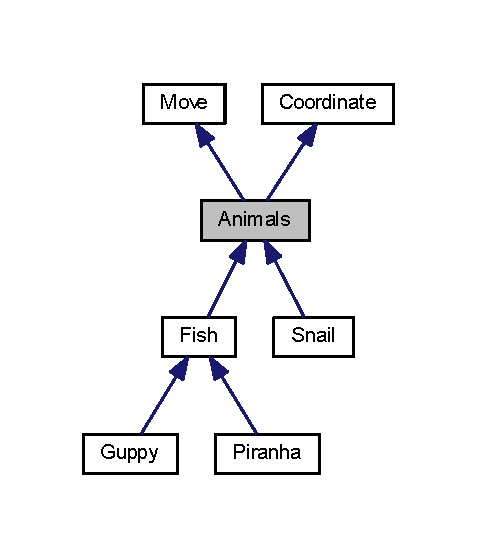
\includegraphics[width=229pt]{class_animals__inherit__graph}
\end{center}
\end{figure}


Collaboration diagram for Animals\+:
\nopagebreak
\begin{figure}[H]
\begin{center}
\leavevmode
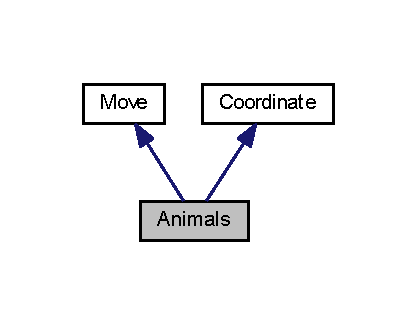
\includegraphics[width=200pt]{class_animals__coll__graph}
\end{center}
\end{figure}
\subsection*{Public Member Functions}
\begin{DoxyCompactItemize}
\item 
\mbox{\Hypertarget{class_animals_ac1a5ca3b403377125688fdc8687db721}\label{class_animals_ac1a5ca3b403377125688fdc8687db721}} 
{\bfseries Animals} (int x, int y, int speed)
\item 
\mbox{\Hypertarget{class_animals_adbd7dbb6d8bd178fc983dbaf34ff0c41}\label{class_animals_adbd7dbb6d8bd178fc983dbaf34ff0c41}} 
virtual void {\bfseries eat} ()=0
\item 
\mbox{\Hypertarget{class_animals_a38b3b917bcd3e7af6e408ae91a1e51ab}\label{class_animals_a38b3b917bcd3e7af6e408ae91a1e51ab}} 
virtual void {\bfseries synchronize} ()=0
\item 
\mbox{\Hypertarget{class_animals_a04d055b9a5a78eecd78cb6715a3ba32b}\label{class_animals_a04d055b9a5a78eecd78cb6715a3ba32b}} 
int {\bfseries get\+Speed} ()
\item 
\mbox{\Hypertarget{class_animals_a2efba71e156ee08d8e16099ab59de23c}\label{class_animals_a2efba71e156ee08d8e16099ab59de23c}} 
void {\bfseries set\+Speed} (int speed)
\end{DoxyCompactItemize}


The documentation for this class was generated from the following file\+:\begin{DoxyCompactItemize}
\item 
Animals.\+h\end{DoxyCompactItemize}

\hypertarget{class_aquarium}{}\section{Aquarium Class Reference}
\label{class_aquarium}\index{Aquarium@{Aquarium}}
\subsection*{Public Member Functions}
\begin{DoxyCompactItemize}
\item 
\mbox{\Hypertarget{class_aquarium_afc3769b98e225080f88cc3506967630b}\label{class_aquarium_afc3769b98e225080f88cc3506967630b}} 
{\bfseries Aquarium} (int length, int width)
\item 
\mbox{\Hypertarget{class_aquarium_a5545a351928f1669894a4e3ce8c991c7}\label{class_aquarium_a5545a351928f1669894a4e3ce8c991c7}} 
void {\bfseries initiate\+Map} ()
\item 
\mbox{\Hypertarget{class_aquarium_a6697d309ab83f5f29942c78abae302f9}\label{class_aquarium_a6697d309ab83f5f29942c78abae302f9}} 
void {\bfseries next\+Lifetime} ()
\item 
\mbox{\Hypertarget{class_aquarium_a8e6a73c98176e993a633d1da303ee0a9}\label{class_aquarium_a8e6a73c98176e993a633d1da303ee0a9}} 
void {\bfseries add\+Guppy} ()
\item 
\mbox{\Hypertarget{class_aquarium_a78cf0346acc80cb65c09c3e71b853921}\label{class_aquarium_a78cf0346acc80cb65c09c3e71b853921}} 
void {\bfseries add\+Piranha} ()
\item 
\mbox{\Hypertarget{class_aquarium_a9e14c2ba9addcf10c5cc68ff910ac387}\label{class_aquarium_a9e14c2ba9addcf10c5cc68ff910ac387}} 
void {\bfseries add\+Coin} ()
\item 
\mbox{\Hypertarget{class_aquarium_a2182e36f0ee4440eeb7837e9ccb32eae}\label{class_aquarium_a2182e36f0ee4440eeb7837e9ccb32eae}} 
void {\bfseries add\+Fish\+Food} ()
\item 
\mbox{\Hypertarget{class_aquarium_a2c17ac30fcdf6fd392df069a347461c4}\label{class_aquarium_a2c17ac30fcdf6fd392df069a347461c4}} 
int {\bfseries get\+Aquarium\+Lifetime} ()
\item 
\mbox{\Hypertarget{class_aquarium_a6e6dbecee1ec13aaf052ac51ea611f88}\label{class_aquarium_a6e6dbecee1ec13aaf052ac51ea611f88}} 
void {\bfseries set\+Aquarium\+Lifetime} (int lifetime)
\end{DoxyCompactItemize}
\subsection*{Static Public Attributes}
\begin{DoxyCompactItemize}
\item 
\mbox{\Hypertarget{class_aquarium_ab1b494ef184b67398018b7727244dab7}\label{class_aquarium_ab1b494ef184b67398018b7727244dab7}} 
static int {\bfseries aquarium\+Coin} = 10
\end{DoxyCompactItemize}


The documentation for this class was generated from the following file\+:\begin{DoxyCompactItemize}
\item 
Aquarium.\+h\end{DoxyCompactItemize}

\hypertarget{class_coin}{}\section{Coin Class Reference}
\label{class_coin}\index{Coin@{Coin}}


Inheritance diagram for Coin\+:
\nopagebreak
\begin{figure}[H]
\begin{center}
\leavevmode
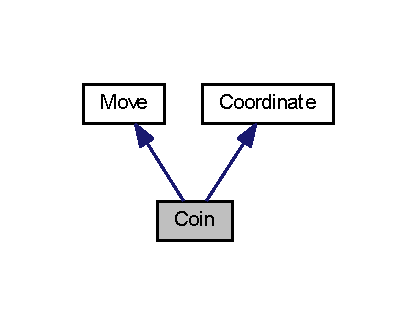
\includegraphics[width=200pt]{class_coin__inherit__graph}
\end{center}
\end{figure}


Collaboration diagram for Coin\+:
\nopagebreak
\begin{figure}[H]
\begin{center}
\leavevmode
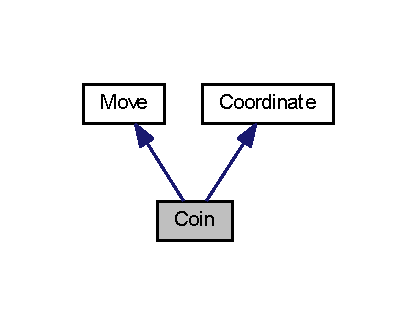
\includegraphics[width=200pt]{class_coin__coll__graph}
\end{center}
\end{figure}
\subsection*{Public Member Functions}
\begin{DoxyCompactItemize}
\item 
\mbox{\Hypertarget{class_coin_a5e902f1d885451d7ccaee72737519473}\label{class_coin_a5e902f1d885451d7ccaee72737519473}} 
{\bfseries Coin} (int x, int y, int value, int speed)
\item 
\mbox{\Hypertarget{class_coin_a223ac1d0cdf80c8eca9bd09edfc0edbc}\label{class_coin_a223ac1d0cdf80c8eca9bd09edfc0edbc}} 
int {\bfseries get\+Speed} ()
\item 
\mbox{\Hypertarget{class_coin_a0b367a3b902b5c2a4787706fa5a13972}\label{class_coin_a0b367a3b902b5c2a4787706fa5a13972}} 
void {\bfseries set\+Speed} (int speed)
\item 
\mbox{\Hypertarget{class_coin_a644f624bd7da3210cb040f3bdb87b226}\label{class_coin_a644f624bd7da3210cb040f3bdb87b226}} 
void {\bfseries move\+Bottom} ()
\item 
\mbox{\Hypertarget{class_coin_ae12c00f84a81afbb7edb2aa3b9842683}\label{class_coin_ae12c00f84a81afbb7edb2aa3b9842683}} 
bool {\bfseries operator==} (const \mbox{\hyperlink{class_coin}{Coin}} \&C)
\end{DoxyCompactItemize}


The documentation for this class was generated from the following file\+:\begin{DoxyCompactItemize}
\item 
Coin.\+h\end{DoxyCompactItemize}

\hypertarget{class_coordinate}{}\section{Coordinate Class Reference}
\label{class_coordinate}\index{Coordinate@{Coordinate}}


Inheritance diagram for Coordinate\+:
\nopagebreak
\begin{figure}[H]
\begin{center}
\leavevmode
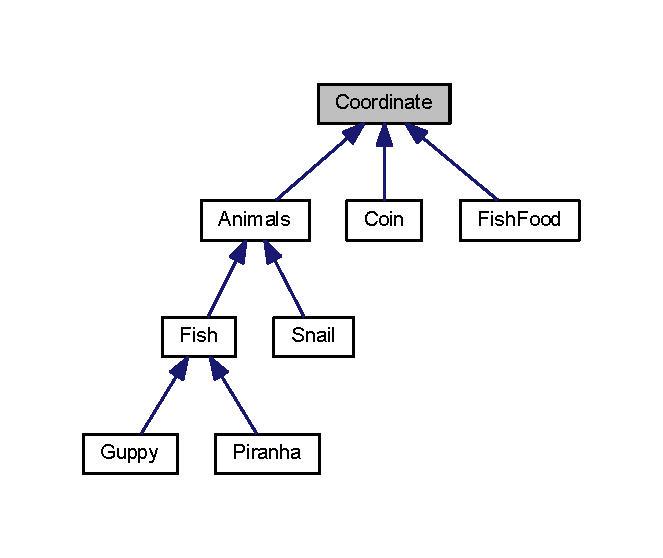
\includegraphics[width=318pt]{class_coordinate__inherit__graph}
\end{center}
\end{figure}
\subsection*{Public Member Functions}
\begin{DoxyCompactItemize}
\item 
\mbox{\Hypertarget{class_coordinate_aba3fc03b1a25f335c9058ddf18290d59}\label{class_coordinate_aba3fc03b1a25f335c9058ddf18290d59}} 
{\bfseries Coordinate} (int x, int y)
\item 
\mbox{\Hypertarget{class_coordinate_ac093fddac8f2c633b1c64b441bbfc6e2}\label{class_coordinate_ac093fddac8f2c633b1c64b441bbfc6e2}} 
int {\bfseries getX} ()
\item 
\mbox{\Hypertarget{class_coordinate_aa2972c516f1c636f4f2bfa92042a8ff2}\label{class_coordinate_aa2972c516f1c636f4f2bfa92042a8ff2}} 
int {\bfseries getY} ()
\item 
\mbox{\Hypertarget{class_coordinate_ad5dbae717bf274df8b7e13b5640a9472}\label{class_coordinate_ad5dbae717bf274df8b7e13b5640a9472}} 
void {\bfseries setX} (int x)
\item 
\mbox{\Hypertarget{class_coordinate_a0375bac44bb4d6950e829a3d1560830a}\label{class_coordinate_a0375bac44bb4d6950e829a3d1560830a}} 
void {\bfseries setY} (int y)
\end{DoxyCompactItemize}


The documentation for this class was generated from the following file\+:\begin{DoxyCompactItemize}
\item 
Coordinate.\+h\end{DoxyCompactItemize}

\hypertarget{class_fish}{}\section{Fish Class Reference}
\label{class_fish}\index{Fish@{Fish}}


Inheritance diagram for Fish\+:
\nopagebreak
\begin{figure}[H]
\begin{center}
\leavevmode
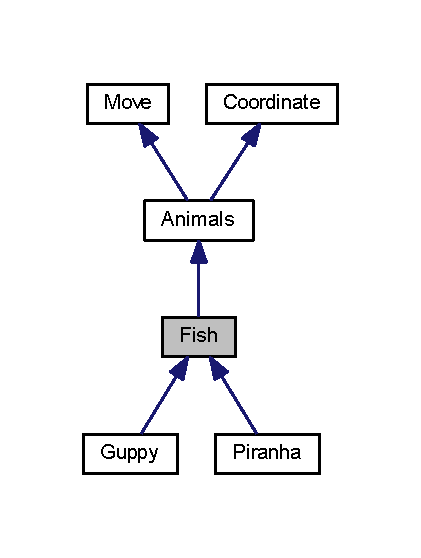
\includegraphics[width=202pt]{class_fish__inherit__graph}
\end{center}
\end{figure}


Collaboration diagram for Fish\+:
\nopagebreak
\begin{figure}[H]
\begin{center}
\leavevmode
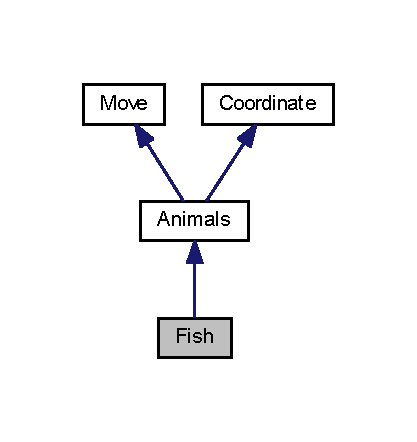
\includegraphics[width=200pt]{class_fish__coll__graph}
\end{center}
\end{figure}
\subsection*{Public Member Functions}
\begin{DoxyCompactItemize}
\item 
\mbox{\Hypertarget{class_fish_a1cad2923de843048dab6908d7e11bb00}\label{class_fish_a1cad2923de843048dab6908d7e11bb00}} 
{\bfseries Fish} (int x, int y, int speed)
\item 
\mbox{\Hypertarget{class_fish_ac4e2bc7d1c0df07728685ae78d7764b4}\label{class_fish_ac4e2bc7d1c0df07728685ae78d7764b4}} 
int {\bfseries get\+Id} ()
\item 
\mbox{\Hypertarget{class_fish_af796997e3f6aa164e9c461e4eab54f3b}\label{class_fish_af796997e3f6aa164e9c461e4eab54f3b}} 
int {\bfseries get\+Lifetime} ()
\item 
\mbox{\Hypertarget{class_fish_a2f3e5915d95a6c22bb8290e046e84676}\label{class_fish_a2f3e5915d95a6c22bb8290e046e84676}} 
int {\bfseries get\+Still\+Full} ()
\item 
\mbox{\Hypertarget{class_fish_a5eeb331c3feaf879836138dc423a29a7}\label{class_fish_a5eeb331c3feaf879836138dc423a29a7}} 
int {\bfseries get\+Counting\+Dead} ()
\item 
\mbox{\Hypertarget{class_fish_a5ff69256c70ab85c6cfefa7767116c63}\label{class_fish_a5ff69256c70ab85c6cfefa7767116c63}} 
int {\bfseries get\+Look\+At} ()
\item 
\mbox{\Hypertarget{class_fish_a318f36bb4023d32c93f1c31ba6714157}\label{class_fish_a318f36bb4023d32c93f1c31ba6714157}} 
void {\bfseries set\+Id} (int id)
\item 
\mbox{\Hypertarget{class_fish_ad7e9032a5f826714df0d9b644fb11a8a}\label{class_fish_ad7e9032a5f826714df0d9b644fb11a8a}} 
void {\bfseries set\+Lifetime} (int lifetime)
\item 
\mbox{\Hypertarget{class_fish_a6c7ce1e1489f4cac6fbf2218af198585}\label{class_fish_a6c7ce1e1489f4cac6fbf2218af198585}} 
void {\bfseries set\+Still\+Full} (int still\+Full)
\item 
\mbox{\Hypertarget{class_fish_ab8aab50eb6109450eb478149b1aa0b62}\label{class_fish_ab8aab50eb6109450eb478149b1aa0b62}} 
void {\bfseries set\+Counting\+Dead} (int counting\+Dead)
\item 
\mbox{\Hypertarget{class_fish_a8bcf2c1da07a83c9c3964e3550434f80}\label{class_fish_a8bcf2c1da07a83c9c3964e3550434f80}} 
void {\bfseries set\+Look\+At} (int look\+At)
\item 
\mbox{\Hypertarget{class_fish_adb64e0ebd369fa4e8d6103cb46362e4b}\label{class_fish_adb64e0ebd369fa4e8d6103cb46362e4b}} 
bool {\bfseries not\+Hungry} ()
\item 
\mbox{\Hypertarget{class_fish_aa93ccf117491c6778c0ab3eb5b454997}\label{class_fish_aa93ccf117491c6778c0ab3eb5b454997}} 
bool {\bfseries is\+Dead} ()
\item 
\mbox{\Hypertarget{class_fish_a54eadea82441af699651d73b877ba178}\label{class_fish_a54eadea82441af699651d73b877ba178}} 
virtual \mbox{\hyperlink{class_coin}{Coin}} {\bfseries make\+Coin} ()=0
\item 
\mbox{\Hypertarget{class_fish_a25946c0d81cd0edd1e22762f7b34e16b}\label{class_fish_a25946c0d81cd0edd1e22762f7b34e16b}} 
void {\bfseries move} (int direction)
\item 
\mbox{\Hypertarget{class_fish_a578f11894521e56ddbd62c30ef1dfe8d}\label{class_fish_a578f11894521e56ddbd62c30ef1dfe8d}} 
void {\bfseries move\+Top} ()
\item 
\mbox{\Hypertarget{class_fish_ac2cceb1e9b353522909d81d7071a9595}\label{class_fish_ac2cceb1e9b353522909d81d7071a9595}} 
void {\bfseries move\+Bottom} ()
\item 
\mbox{\Hypertarget{class_fish_ab8a55c0af173c7af006952fa47b08b7a}\label{class_fish_ab8a55c0af173c7af006952fa47b08b7a}} 
void {\bfseries move\+Right} ()
\item 
\mbox{\Hypertarget{class_fish_a440c300548c92ffdd4582c62beccc95e}\label{class_fish_a440c300548c92ffdd4582c62beccc95e}} 
void {\bfseries move\+Left} ()
\item 
\mbox{\Hypertarget{class_fish_af895191e0ccaf45fca80f62913db642d}\label{class_fish_af895191e0ccaf45fca80f62913db642d}} 
void {\bfseries move\+Diagonal\+Top\+Left} ()
\item 
\mbox{\Hypertarget{class_fish_ae76c1f17dbf67a93d1f7ab461a11171f}\label{class_fish_ae76c1f17dbf67a93d1f7ab461a11171f}} 
void {\bfseries move\+Diagonal\+Top\+Right} ()
\item 
\mbox{\Hypertarget{class_fish_a7b9ea9778f079638e0e1b1bd5263aa5d}\label{class_fish_a7b9ea9778f079638e0e1b1bd5263aa5d}} 
void {\bfseries move\+Diagonal\+Bottom\+Right} ()
\item 
\mbox{\Hypertarget{class_fish_a26f6c324a4081bcfd9fbb8770031b13c}\label{class_fish_a26f6c324a4081bcfd9fbb8770031b13c}} 
void {\bfseries move\+Diagonal\+Bottom\+Left} ()
\item 
\mbox{\Hypertarget{class_fish_a7473acf2b44fc41c1741a98a9a1c4038}\label{class_fish_a7473acf2b44fc41c1741a98a9a1c4038}} 
void {\bfseries synchronize} ()
\item 
\mbox{\Hypertarget{class_fish_a972444e9ae06cf53ea0823447eb79508}\label{class_fish_a972444e9ae06cf53ea0823447eb79508}} 
void {\bfseries dead} ()
\end{DoxyCompactItemize}


The documentation for this class was generated from the following file\+:\begin{DoxyCompactItemize}
\item 
Fish.\+h\end{DoxyCompactItemize}

\hypertarget{class_fish_food}{}\section{Fish\+Food Class Reference}
\label{class_fish_food}\index{Fish\+Food@{Fish\+Food}}


Inheritance diagram for Fish\+Food\+:
\nopagebreak
\begin{figure}[H]
\begin{center}
\leavevmode
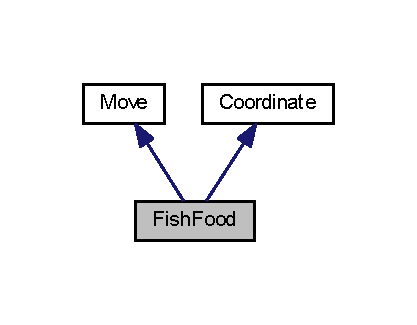
\includegraphics[width=200pt]{class_fish_food__inherit__graph}
\end{center}
\end{figure}


Collaboration diagram for Fish\+Food\+:
\nopagebreak
\begin{figure}[H]
\begin{center}
\leavevmode
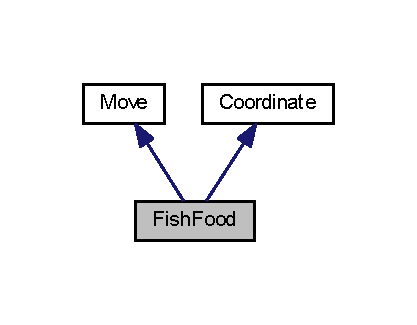
\includegraphics[width=200pt]{class_fish_food__coll__graph}
\end{center}
\end{figure}
\subsection*{Public Member Functions}
\begin{DoxyCompactItemize}
\item 
\mbox{\Hypertarget{class_fish_food_ae5d65712b4a210fb0d0b4b7ff73437a4}\label{class_fish_food_ae5d65712b4a210fb0d0b4b7ff73437a4}} 
{\bfseries Fish\+Food} (int x, int y, int speed)
\item 
\mbox{\Hypertarget{class_fish_food_a80b014bc6c50a1ff587f370deea1d7e1}\label{class_fish_food_a80b014bc6c50a1ff587f370deea1d7e1}} 
int {\bfseries get\+Speed} ()
\item 
\mbox{\Hypertarget{class_fish_food_a3451d81067fbdd80cb56a86ff8e8d2b4}\label{class_fish_food_a3451d81067fbdd80cb56a86ff8e8d2b4}} 
void {\bfseries set\+Speed} (int speed)
\item 
\mbox{\Hypertarget{class_fish_food_a82804b517124060d60ddd983d6e986ba}\label{class_fish_food_a82804b517124060d60ddd983d6e986ba}} 
void {\bfseries move\+Bottom} ()
\item 
\mbox{\Hypertarget{class_fish_food_a1a6fccff6e7b76ab5ab4840f09de2967}\label{class_fish_food_a1a6fccff6e7b76ab5ab4840f09de2967}} 
bool {\bfseries operator==} (const \mbox{\hyperlink{class_fish_food}{Fish\+Food}} \&F)
\end{DoxyCompactItemize}


The documentation for this class was generated from the following file\+:\begin{DoxyCompactItemize}
\item 
Fish\+Food.\+h\end{DoxyCompactItemize}

\hypertarget{class_guppy}{}\section{Guppy Class Reference}
\label{class_guppy}\index{Guppy@{Guppy}}


Inheritance diagram for Guppy\+:
\nopagebreak
\begin{figure}[H]
\begin{center}
\leavevmode
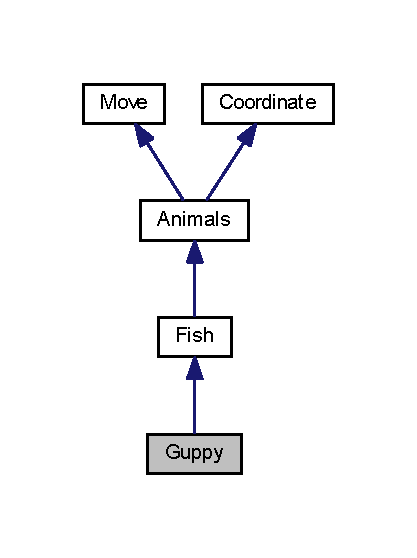
\includegraphics[width=200pt]{class_guppy__inherit__graph}
\end{center}
\end{figure}


Collaboration diagram for Guppy\+:
\nopagebreak
\begin{figure}[H]
\begin{center}
\leavevmode
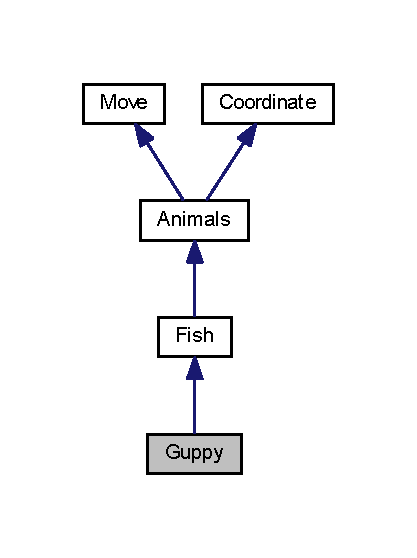
\includegraphics[width=200pt]{class_guppy__coll__graph}
\end{center}
\end{figure}
\subsection*{Public Member Functions}
\begin{DoxyCompactItemize}
\item 
\mbox{\Hypertarget{class_guppy_a8b7a9abdd40f669b4e84b66d0cf403ef}\label{class_guppy_a8b7a9abdd40f669b4e84b66d0cf403ef}} 
{\bfseries Guppy} (int x, int y)
\item 
\mbox{\Hypertarget{class_guppy_a02efb73289d3b94264fba7d6c1d985b8}\label{class_guppy_a02efb73289d3b94264fba7d6c1d985b8}} 
bool {\bfseries operator==} (const \mbox{\hyperlink{class_guppy}{Guppy}} \&G)
\item 
\mbox{\Hypertarget{class_guppy_a77d65bb4c13bbd85d4acd65f11a21b9e}\label{class_guppy_a77d65bb4c13bbd85d4acd65f11a21b9e}} 
int {\bfseries get\+Phase} ()
\item 
\mbox{\Hypertarget{class_guppy_afe934262a0988e4ad041f4ed3a1a7e02}\label{class_guppy_afe934262a0988e4ad041f4ed3a1a7e02}} 
void {\bfseries eat} ()
\item 
\mbox{\Hypertarget{class_guppy_abb939e91eb5b9b1609cc0b78ec1bd4b2}\label{class_guppy_abb939e91eb5b9b1609cc0b78ec1bd4b2}} 
\mbox{\hyperlink{class_coin}{Coin}} {\bfseries make\+Coin} ()
\item 
\mbox{\Hypertarget{class_guppy_af05a02b3c902ab272e775d6b4dd33ef3}\label{class_guppy_af05a02b3c902ab272e775d6b4dd33ef3}} 
void {\bfseries next\+Phase} ()
\item 
\mbox{\Hypertarget{class_guppy_ae26531e81083050c4fab3b3358b49cc5}\label{class_guppy_ae26531e81083050c4fab3b3358b49cc5}} 
\mbox{\hyperlink{class_fish_food}{Fish\+Food}} {\bfseries get\+Nearest\+Food} (\mbox{\hyperlink{class_linked_list}{Linked\+List}}$<$ \mbox{\hyperlink{class_fish_food}{Fish\+Food}} $>$ list\+Food)
\end{DoxyCompactItemize}


The documentation for this class was generated from the following file\+:\begin{DoxyCompactItemize}
\item 
Guppy.\+h\end{DoxyCompactItemize}

\hypertarget{class_linked_list}{}\section{Linked\+List$<$ T $>$ Class Template Reference}
\label{class_linked_list}\index{Linked\+List$<$ T $>$@{Linked\+List$<$ T $>$}}
\subsection*{Public Member Functions}
\begin{DoxyCompactItemize}
\item 
\mbox{\Hypertarget{class_linked_list_af9b832a7649af3c40420782ecef9e205}\label{class_linked_list_af9b832a7649af3c40420782ecef9e205}} 
{\bfseries Linked\+List} (T data)
\item 
\mbox{\Hypertarget{class_linked_list_a7ecbb28e82117a680839ed0dc28ebdce}\label{class_linked_list_a7ecbb28e82117a680839ed0dc28ebdce}} 
bool {\bfseries is\+Empty} ()
\item 
\mbox{\Hypertarget{class_linked_list_ab7364799e5965dd59d4f5952cb953287}\label{class_linked_list_ab7364799e5965dd59d4f5952cb953287}} 
void {\bfseries add} (T element)
\item 
\mbox{\Hypertarget{class_linked_list_a6c4973ae9956ddb037a9093cffa2adb1}\label{class_linked_list_a6c4973ae9956ddb037a9093cffa2adb1}} 
void {\bfseries remove} (T element)
\item 
\mbox{\Hypertarget{class_linked_list_a25079ed9b408efad63a1522c818d8705}\label{class_linked_list_a25079ed9b408efad63a1522c818d8705}} 
T {\bfseries get} (int index)
\end{DoxyCompactItemize}


The documentation for this class was generated from the following file\+:\begin{DoxyCompactItemize}
\item 
Linked\+List.\+h\end{DoxyCompactItemize}

\hypertarget{class_move}{}\section{Move Class Reference}
\label{class_move}\index{Move@{Move}}


Inheritance diagram for Move\+:
\nopagebreak
\begin{figure}[H]
\begin{center}
\leavevmode
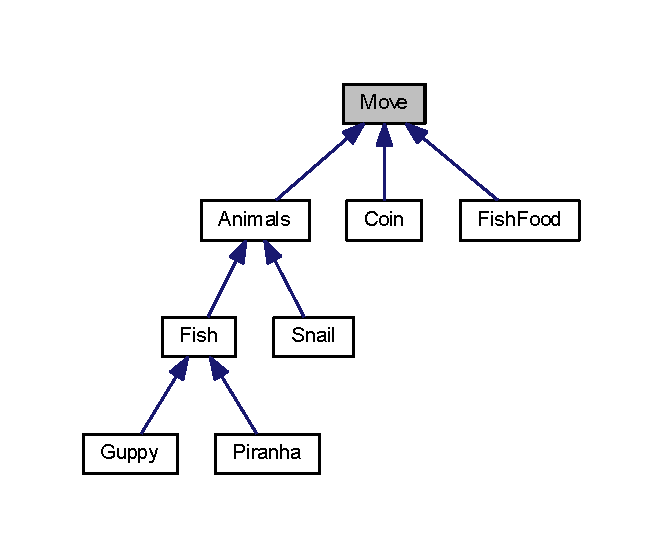
\includegraphics[width=318pt]{class_move__inherit__graph}
\end{center}
\end{figure}
\subsection*{Public Member Functions}
\begin{DoxyCompactItemize}
\item 
\mbox{\Hypertarget{class_move_ada092c8b3ab8e9c6824432a04dbad285}\label{class_move_ada092c8b3ab8e9c6824432a04dbad285}} 
virtual void {\bfseries move\+Top} ()=0
\item 
\mbox{\Hypertarget{class_move_a183afa5e8eb4efb49f30675fd60ccceb}\label{class_move_a183afa5e8eb4efb49f30675fd60ccceb}} 
virtual void {\bfseries move\+Bottom} ()=0
\item 
\mbox{\Hypertarget{class_move_af147ff62b7d9789da1b5d08958a90d39}\label{class_move_af147ff62b7d9789da1b5d08958a90d39}} 
virtual void {\bfseries move\+Right} ()=0
\item 
\mbox{\Hypertarget{class_move_aa7cd66ebda7f528c42a864c6a656d7d5}\label{class_move_aa7cd66ebda7f528c42a864c6a656d7d5}} 
virtual void {\bfseries move\+Left} ()=0
\item 
\mbox{\Hypertarget{class_move_a3b2c83c3735c10ab11fe809fc0d34b19}\label{class_move_a3b2c83c3735c10ab11fe809fc0d34b19}} 
virtual void {\bfseries move\+Diagonal\+Top\+Left} ()=0
\item 
\mbox{\Hypertarget{class_move_a9696ef666d5526fab259215275f66647}\label{class_move_a9696ef666d5526fab259215275f66647}} 
virtual void {\bfseries move\+Diagonal\+Top\+Right} ()=0
\item 
\mbox{\Hypertarget{class_move_ae05211234da445f809c862492abcbce1}\label{class_move_ae05211234da445f809c862492abcbce1}} 
virtual void {\bfseries move\+Diagonal\+Bottom\+Right} ()=0
\item 
\mbox{\Hypertarget{class_move_a8c9bf0880455645406acbbf0d426ea38}\label{class_move_a8c9bf0880455645406acbbf0d426ea38}} 
virtual void {\bfseries move\+Diagonal\+Bottom\+Left} ()=0
\end{DoxyCompactItemize}


The documentation for this class was generated from the following file\+:\begin{DoxyCompactItemize}
\item 
Move.\+h\end{DoxyCompactItemize}

\hypertarget{class_piranha}{}\section{Piranha Class Reference}
\label{class_piranha}\index{Piranha@{Piranha}}


Inheritance diagram for Piranha\+:
\nopagebreak
\begin{figure}[H]
\begin{center}
\leavevmode
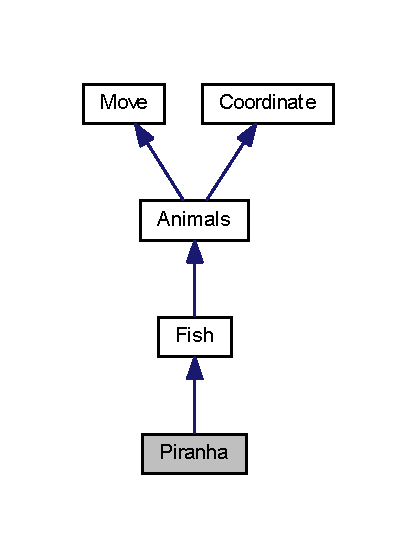
\includegraphics[width=200pt]{class_piranha__inherit__graph}
\end{center}
\end{figure}


Collaboration diagram for Piranha\+:
\nopagebreak
\begin{figure}[H]
\begin{center}
\leavevmode
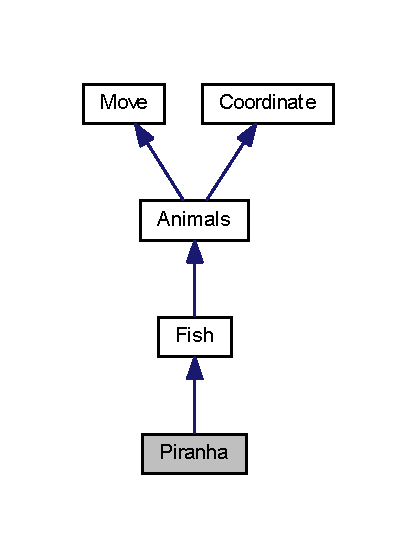
\includegraphics[width=200pt]{class_piranha__coll__graph}
\end{center}
\end{figure}
\subsection*{Public Member Functions}
\begin{DoxyCompactItemize}
\item 
\mbox{\Hypertarget{class_piranha_a78b80929a5c5d8e1d82477026fb1a1e9}\label{class_piranha_a78b80929a5c5d8e1d82477026fb1a1e9}} 
{\bfseries Piranha} (int x, int y)
\item 
\mbox{\Hypertarget{class_piranha_a3c16f356d1f90a0ca33caa0d5cc8f931}\label{class_piranha_a3c16f356d1f90a0ca33caa0d5cc8f931}} 
bool {\bfseries operator==} (const \mbox{\hyperlink{class_piranha}{Piranha}} \&G)
\item 
\mbox{\Hypertarget{class_piranha_ac48c0256edd56c427b3d82f6e0d4df82}\label{class_piranha_ac48c0256edd56c427b3d82f6e0d4df82}} 
void {\bfseries eat} ()
\item 
\mbox{\Hypertarget{class_piranha_a288fe5baeae95af1ce3afaae77f3bf1d}\label{class_piranha_a288fe5baeae95af1ce3afaae77f3bf1d}} 
\mbox{\hyperlink{class_coin}{Coin}} {\bfseries make\+Coin} ()
\item 
\mbox{\Hypertarget{class_piranha_a93ba25800a80842e52e42adaede6aae0}\label{class_piranha_a93ba25800a80842e52e42adaede6aae0}} 
\mbox{\hyperlink{class_guppy}{Guppy}} {\bfseries get\+Nearest\+Guppy} (\mbox{\hyperlink{class_linked_list}{Linked\+List}}$<$ \mbox{\hyperlink{class_guppy}{Guppy}} $>$ list\+Guppy)
\end{DoxyCompactItemize}


The documentation for this class was generated from the following file\+:\begin{DoxyCompactItemize}
\item 
Piranha.\+h\end{DoxyCompactItemize}

\hypertarget{class_snail}{}\section{Snail Class Reference}
\label{class_snail}\index{Snail@{Snail}}


Inheritance diagram for Snail\+:
\nopagebreak
\begin{figure}[H]
\begin{center}
\leavevmode
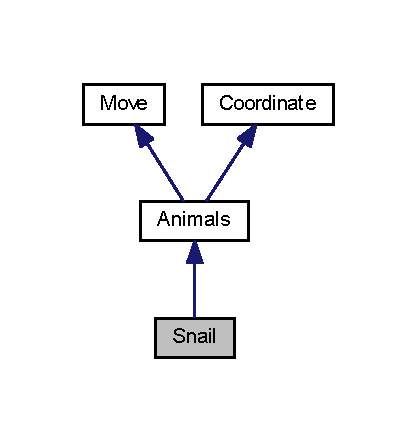
\includegraphics[width=200pt]{class_snail__inherit__graph}
\end{center}
\end{figure}


Collaboration diagram for Snail\+:
\nopagebreak
\begin{figure}[H]
\begin{center}
\leavevmode
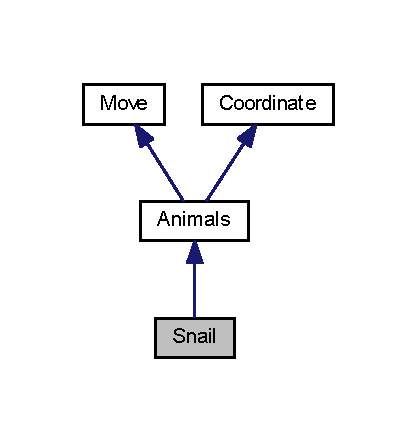
\includegraphics[width=200pt]{class_snail__coll__graph}
\end{center}
\end{figure}
\subsection*{Public Member Functions}
\begin{DoxyCompactItemize}
\item 
\mbox{\Hypertarget{class_snail_af705248e170d76970fe23ac2e5fd2dcd}\label{class_snail_af705248e170d76970fe23ac2e5fd2dcd}} 
{\bfseries Snail} (int x, int y)
\item 
\mbox{\Hypertarget{class_snail_aa1ef66b01bf704babd6004d2fa42aeb1}\label{class_snail_aa1ef66b01bf704babd6004d2fa42aeb1}} 
int {\bfseries get\+Speed} ()
\item 
\mbox{\Hypertarget{class_snail_ab3d472ef9c58dc37a068c34dcee9d355}\label{class_snail_ab3d472ef9c58dc37a068c34dcee9d355}} 
void {\bfseries set\+Speed} (int speed)
\item 
\mbox{\Hypertarget{class_snail_af1d3b378b87936ff924b28223648401c}\label{class_snail_af1d3b378b87936ff924b28223648401c}} 
void {\bfseries eat} ()
\item 
\mbox{\Hypertarget{class_snail_a4c9682f1fc8ac82f98d56de6c8044fbd}\label{class_snail_a4c9682f1fc8ac82f98d56de6c8044fbd}} 
void {\bfseries synchronize} ()
\item 
\mbox{\Hypertarget{class_snail_a5fd9dc10de8c086659cbc223552f15d8}\label{class_snail_a5fd9dc10de8c086659cbc223552f15d8}} 
\mbox{\hyperlink{class_snail}{Snail}} \& {\bfseries operator=} (const \mbox{\hyperlink{class_snail}{Snail}} \&S)
\item 
\mbox{\Hypertarget{class_snail_a934cb74e9bc80fa462d59a03b5e0c5f4}\label{class_snail_a934cb74e9bc80fa462d59a03b5e0c5f4}} 
\mbox{\hyperlink{class_coin}{Coin}} {\bfseries get\+Nearest\+Coin} (\mbox{\hyperlink{class_linked_list}{Linked\+List}}$<$ \mbox{\hyperlink{class_coin}{Coin}} $>$ list\+Coin)
\item 
\mbox{\Hypertarget{class_snail_acb846d48ca1ed10f2051b155fe50f100}\label{class_snail_acb846d48ca1ed10f2051b155fe50f100}} 
void {\bfseries move\+Right} ()
\item 
\mbox{\Hypertarget{class_snail_a061780e0fe57eeb0861b6b7cc442bf92}\label{class_snail_a061780e0fe57eeb0861b6b7cc442bf92}} 
void {\bfseries move\+Left} ()
\end{DoxyCompactItemize}


The documentation for this class was generated from the following file\+:\begin{DoxyCompactItemize}
\item 
Snail.\+h\end{DoxyCompactItemize}

%--- End generated contents ---

% Index
\backmatter
\newpage
\phantomsection
\clearemptydoublepage
\addcontentsline{toc}{chapter}{Index}
\printindex

\end{document}
